\documentclass[a4paper, 12pt]{article}

% Paquetes básicos para idioma y codificación
\usepackage[utf8]{inputenc}
\usepackage[T1]{fontenc}
\usepackage[spanish]{babel}

% Paquete para insertar imágenes
\usepackage{graphicx}

% --- PAQUETE NUEVO PARA FORZAR LA POSICIÓN DE LAS IMÁGENES ---
\usepackage{float} 

% Paquete para que el índice tenga enlaces clickeables
\usepackage[colorlinks=true, linkcolor=black, urlcolor=blue]{hyperref}

% Configuración del título
\title{Memoria de Prácticas: Ingeniería de Servidores}
\author{Juan Reche Aguilar}
\date{\today}

\begin{document}

% Genera la portada con el título
\maketitle
\clearpage % Usamos clearpage en lugar de newpage

\section{Ejercicio 3: Diseño e implementación de un servicio de almacenamiento}

Para garantizar tanto la tolerancia a fallos (alta disponibilidad) como la flexibilidad 
operativa (escalabilidad), se ha optado por implementar una arquitectura de almacenamiento 
en dos capas: un gestor de volúmenes lógicos (LVM) montado sobre un arreglo redundante de 
discos independientes (RAID 5).

\begin{itemize}
    \item \textbf{Capa Física (RAID 5):} Se ha seleccionado el nivel RAID 5 empleando tres discos 
    físicos (sdb, sdc, sdd). Esta configuración ofrece un equilibrio óptimo entre rendimiento, capacidad de 
    almacenamiento y redundancia. Dado que no se concreta qué tan críticos son los datos se opta por RAID 5 
    ya que se ``pierde'' menos espacio. Al utilizar paridad distribuida, el sistema es capaz de 
    soportar el fallo catastrófico de uno de los discos sin pérdida de datos, garantizando 
    la integridad de la información del servidor.

    \item \textbf{Capa Lógica (LVM):} En lugar de formatear directamente el volumen RAID, este se 
    ha inicializado como un Volumen Físico (PV) de LVM. Posteriormente, se ha añadido este PV a 
    un Grupo de Volúmenes (VG) llamado ``vg\_ejercicio''. Dentro de este VG, se ha creado un Volumen Lógico 
    (LV) denominado ``lv\_ejercicio'' que ocupa de primeras 10GB del espacio disponible. 
    Esta capa de abstracción permite una gestión más flexible del almacenamiento, facilitando la expansión o 
    reducción del espacio asignado al volumen lógico sin afectar la estructura física subyacente, 
    eliminando el problema del crecimiento del volumen de datos a almacenar.
\end{itemize}

% Imagen 6
\begin{figure}[H]
    \centering
    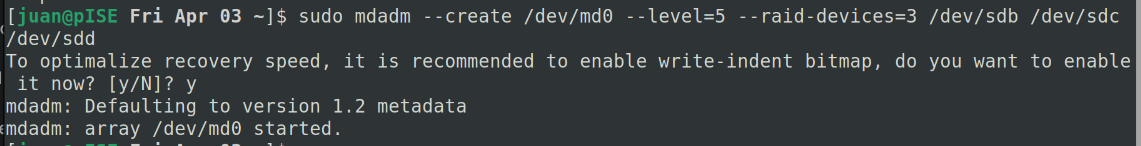
\includegraphics[width=0.8\textwidth]{../ej3/ej3_6.png}
    \caption{Creación del RAID 5 con tres discos fisicos mediante el comando mdadm.}
\end{figure}

% Imagen 7
\begin{figure}[H]
    \centering
    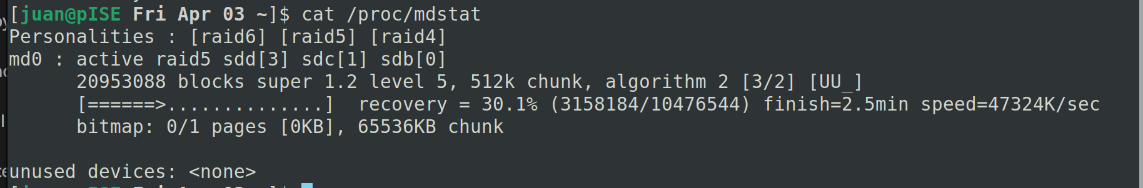
\includegraphics[width=0.8\textwidth]{../ej3/ej3_7.png}
    \caption{Comprobamos que RAID 5 se esta creando}
\end{figure}

% Imagen 8
\begin{figure}[H]
    \centering
    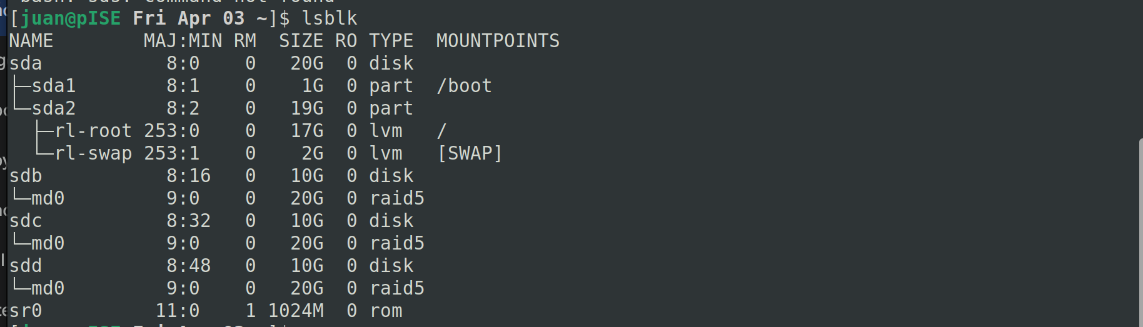
\includegraphics[width=0.8\textwidth]{../ej3/ej3_8.png}
    \caption{Comprobamos que RAID 5 existe}
\end{figure}

% Imagen 9
\begin{figure}[H]
    \centering
    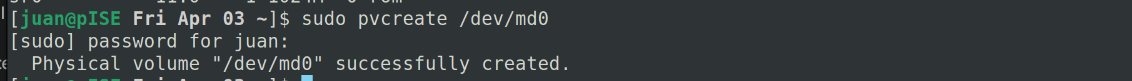
\includegraphics[width=0.8\textwidth]{../ej3/ej3_9.png}
    \caption{Creacion del volumen fisico con el comando pvcreate}
\end{figure}

% Imagen 10
\begin{figure}[H]
    \centering
    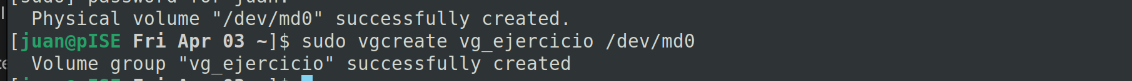
\includegraphics[width=0.8\textwidth]{../ej3/ej3_10.png}
    \caption{Creacion del grupo de volumen con el comando vgcreate}
\end{figure}

% Imagen 11
\begin{figure}[H]
    \centering
    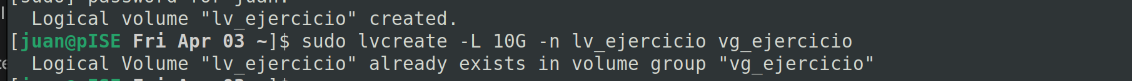
\includegraphics[width=0.8\textwidth]{../ej3/ej3_11.png}
    \caption{Creacion del volumen logico con el comando lvcreate}
\end{figure}

% Imagen 12
\begin{figure}[H]
    \centering
    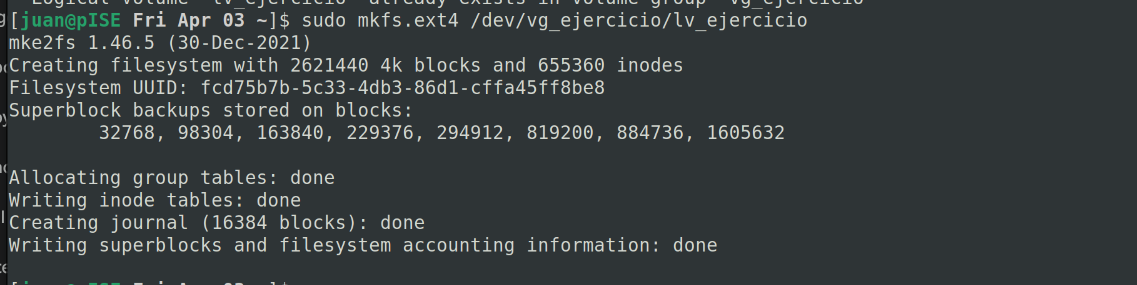
\includegraphics[width=0.8\textwidth]{../ej3/ej3_12.png}
    \caption{Formateamos el volumen logico con el sistema de archivos ext4}
\end{figure}

% Imagen 13
\begin{figure}[H]
    \centering
    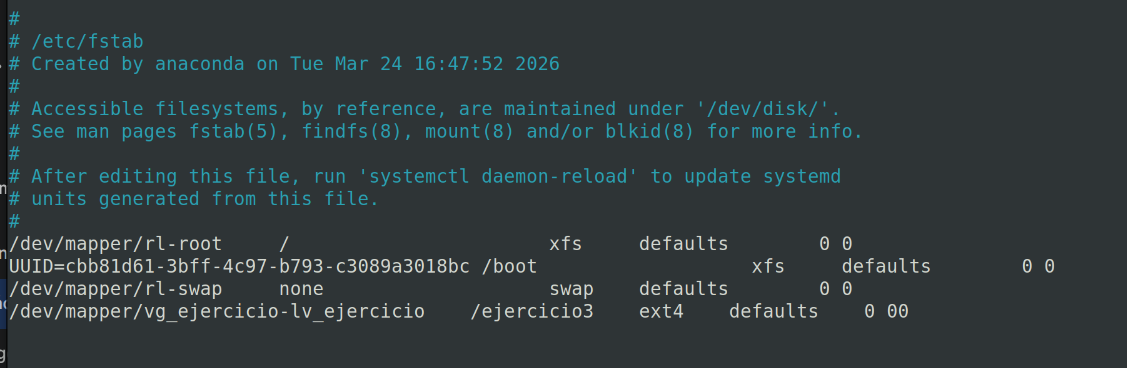
\includegraphics[width=0.8\textwidth]{../ej3/ej3_13.png}
    \caption{Garantizamos la persisistencia del montaje del volumen logico editando el archivo /etc/fstab}
\end{figure}

% Imagen 14
\begin{figure}[H]
    \centering
    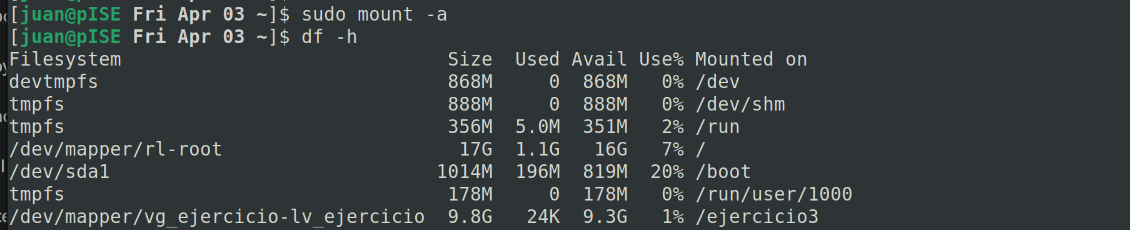
\includegraphics[width=0.8\textwidth]{../ej3/ej3_14.png}
    \caption{Montamos todos los sistemas de archivos del servidor con el comando mount -a 
    y comprobamos la disponibilidad de este nuevo volumen logico con el comando df -h}
\end{figure}

% Imagen 15
\begin{figure}[H]
    \centering
    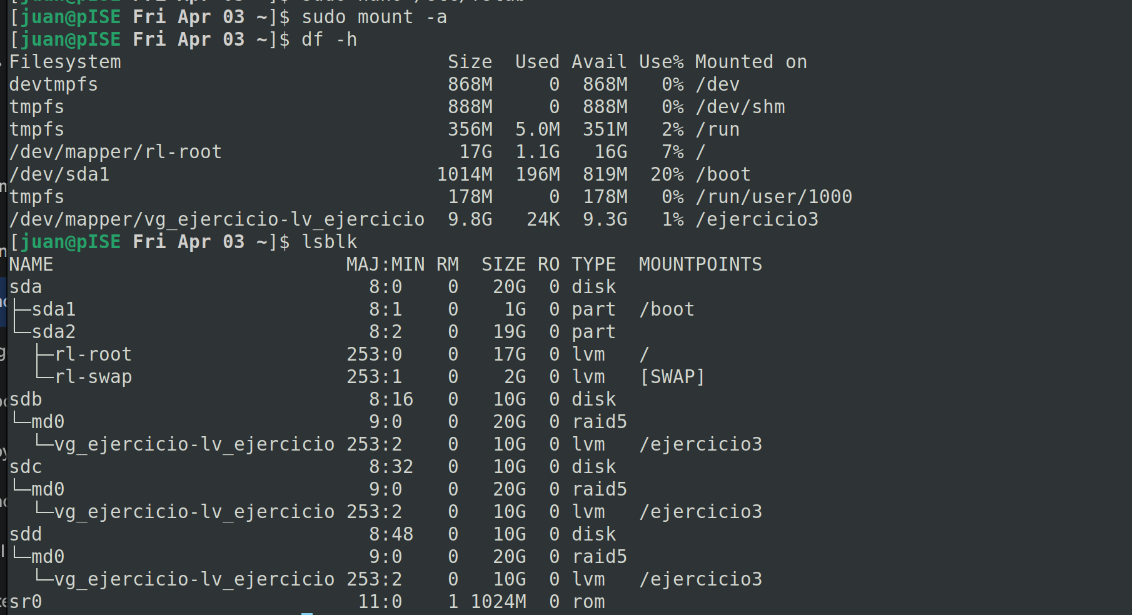
\includegraphics[width=0.8\textwidth]{../ej3/ej3_15.png}
    \caption{Comando final para mostrar el árbol de dispositivos de almacenamiento}
\end{figure}

\end{document}
